\chapter{Data Analysis}
\label{sec:data_analysis}
\section{Data selection and background}
The data analysis has been conducted using Python 3.7. Since the amount of taken data is high 
and only a few events have to be selected, the \textit{Pandas} package \cite{pandas} is 
used to store and handle the data efficiently. \\

The selection is necessary due to the low signal rate in comparison to a high background rate.
Measured trigger signals are not always electron signals from the muon decay.
Since, the experimental setup is positioned inside a building and shielded with a block of iron,
 most of the signals can assumed to originate from muons, since muons are the most penetrating particles. Still, there can be false signals for a variety of reasons. \\

As described in \autoref{sec:trigger} when a muon is stopped by the thinner iron block and thus only produces a signal in P0 and P1. Still, depending on the incoming angle of the muon, a muon can be regarded as stopped even though it is not due to the geometry of this experiment, as shown in \autoref{fig:fake}.

\begin{figure}
	 \centering
	 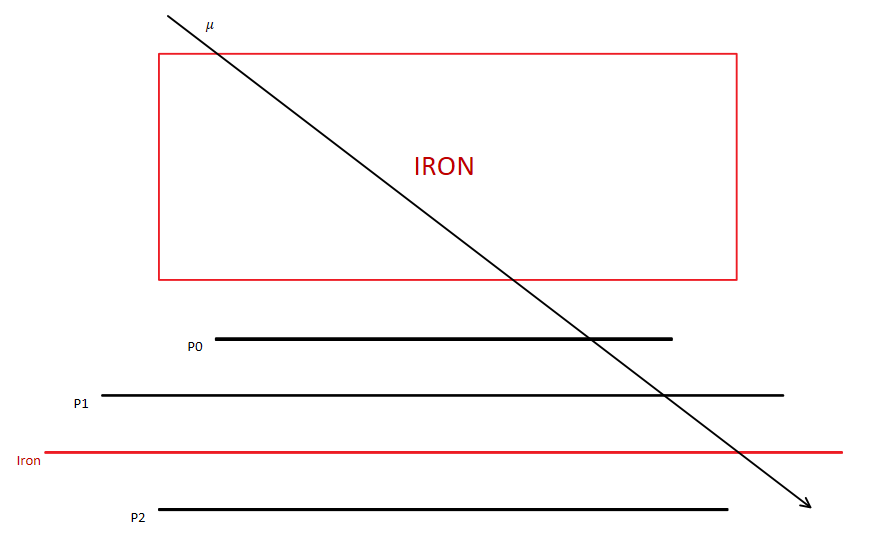
\includegraphics[width=0.6\textwidth]{figures/falsestopping.png}
	 \caption{Scematic of an escaping muon being detected by planes P0 and P1, but not P2 and therefore resulting in a fake trigger signal.}
	 \label{fig:fake}
\end{figure}

In this case, the time measurement starts without a stopped muon. It can affect the measurement in two different ways: firstly, no other particle passes and thus, only overflow values are generated. Secondly, a background signal triggers a channel and produces a fake event.\\

Another possible reason for the background is the correct detection of a stopping muon. But, the electron is not detected because it leaves the detector or does not have enough energy to leave the iron block. This case has shown in \autoref{fig:escape}. And this again leads either to an overflow value or a fake event because of a background signal.

\begin{figure}
	 \centering
	 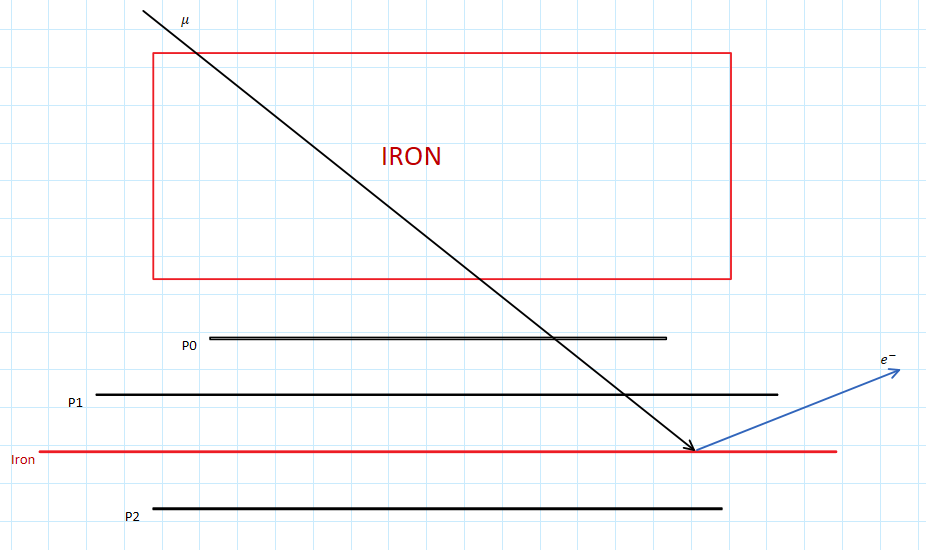
\includegraphics[width=0.6\textwidth]{figures/electron_escape.png}
	 \caption{Scematic of an escaping electron after a muon has stopped. The direction of the decay products is random and so, the electron can escape the detector.}
	 \label{fig:escape}
\end{figure}

These background events can not be eliminated since this experiment does not determine the type of the particle.\\
To handle the analysis, all planes must be looked at separately. This step ensures the statistical independency of all planes, especially for P0 and P1, in which signals often correlate. In the end, all independent analyses were combined for a final result.\\
At first, all overflow values have to eliminate from the data set. The entry for every single plane would considered valid if it has a non-overflow value in the TDC and only detected in this plane.

\section{Fit function}
Particle decay at rest is like every natural spontaneous process, a Poisson distributed process. So the probability for decay after a given time $t$ is represented by a negative exponential probability function
like 
\begin{equation*}
    N(t) = a \cdot \exp(- \frac{t}{\tau})
\end{equation*}

where $N$ is the number of particles and $\tau$ the decay rate.\\ As discussed before background has to be taken into consideration. Since there is no reason to assume the background signals vary over time, so, the distribution of the background will be considered flat. Thus, the complete fit function is 

\begin{equation}
    N(t) = a \cdot \exp\left(- \frac{t}{\tau}\right) + b 
    \label{eqn:fit}
\end{equation}

with the parameter $a$ as a scale factor representing the total amount of particles at $t=0$ ($ a = N(0)$)
and $b$ representing the constant offset due to background signals. The aim of this analysis is to 
find the muon mean lifetime $\tau$. To do this the fit function will be applied to the data of the planes 
using the Python package \textit{scipy} \cite{scipy}.\\
Furthermore, the data of small timescales ($\approx 200\;$ns) will be excluded from this analysis
to reduce the effects of muon capture 
which will be discussed in \autoref{sec:muoncapture}.

\section{Fit results}

At first, all single planes would be analyzed separately after, and all data are taken into account for the final result. All fit results, however, are shown in 
\autoref{tab:data} for a quick overview of the findings. For this analysis, 
decay times up to $8700 \; \symup{ns}$ are taken into account.\\
In the first plane P0, the lowest number of events could be detected which reflects on the resulting lifetime, which is deviates the most from the actual value and has the biggest $\chi^2$-test value.
For P0 a total of 48 bins meaning each bin represents $181.25 \; \symup{ns}$, while the fit is conducted in the inverval $725 \; \symup{ns}$ to $8700 \; \symup{ns}$.
The data and the fitted function for P0 are shown in \autoref{fig:p0}.\\
\begin{figure}
    \centering
    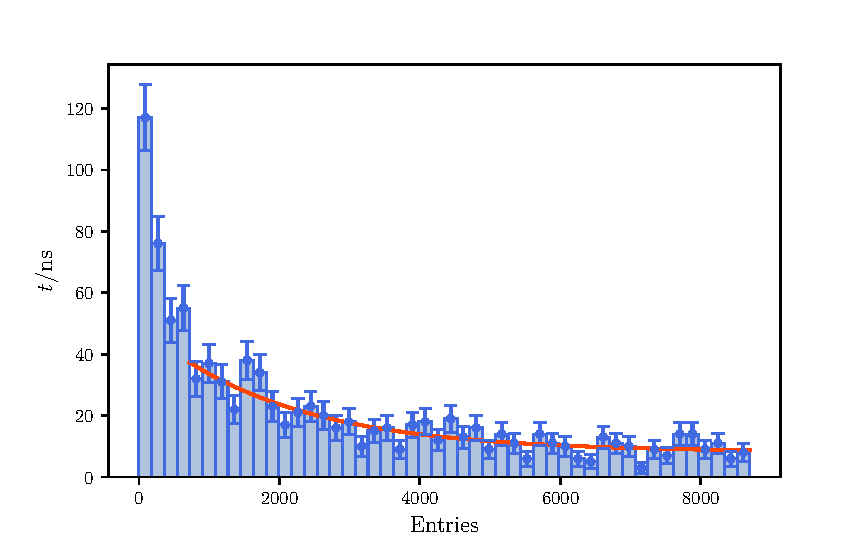
\includegraphics[width=0.6\textwidth]{plots/p0.pdf}
    \caption{Measured events in the plane P0 with plotted decay function.}
    \label{fig:p0}
\end{figure}

The plane P1 measured 2345 events resulting in the lowest $\chi^2$-test value per degree of freedom.
For this plane 77 bins where used with bin sizes of $113 \; \symup{ns}$. The implentation of 
the fit function starts at $226 \; \symup{ns}$. The data and the plotted fit function are shown in \autoref{fig:p1}.\\

\begin{figure}
    \centering
    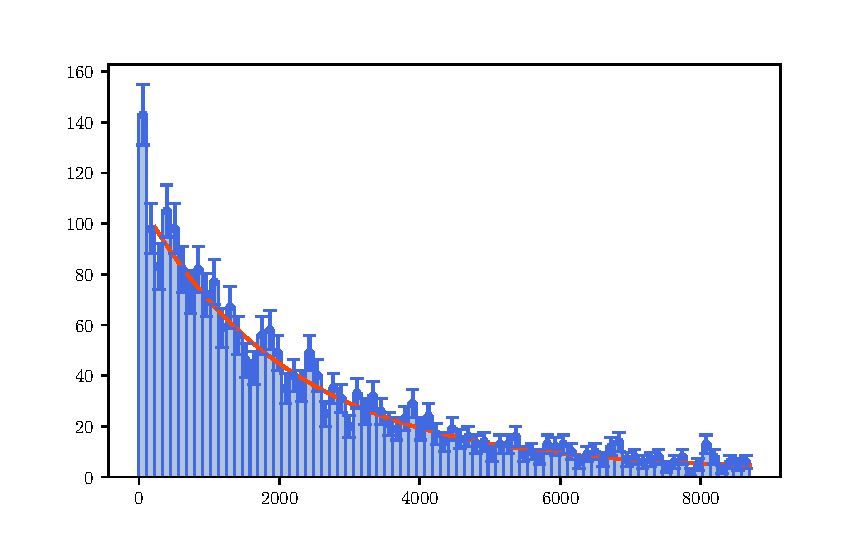
\includegraphics[width=0.6\textwidth]{plots/p1.pdf}
    \caption{Measured events in the plane P1 with plotted decay function.}
    \label{fig:p1}
\end{figure}

For the last plane P2, 60 bins with $145\;\symup{ns}$ are used in the analysis. The fit is conducted 
beginning at $435\;\symup{ns}$. Both data and plotted fit function are shown in \autoref{fig:p2}.\\

\begin{figure}
    \centering
    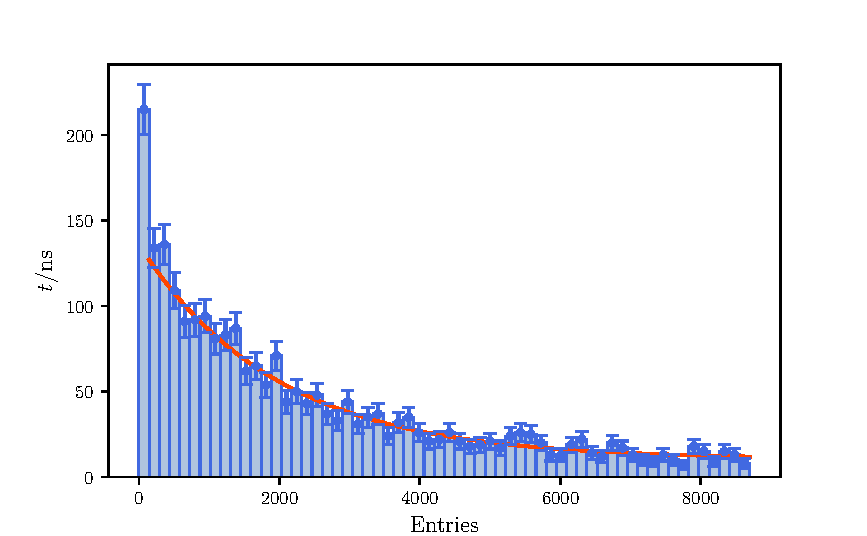
\includegraphics[width=0.6\textwidth]{plots/p2.pdf}
    \caption{Measured events in the plane P2 with plotted decay function.}
    \label{fig:p2}
\end{figure}

Lastly all of the above selected events are considered to gain the highest possible statistic.
Thus, a total amount of 5885 events is taken into consideration. For this analyisis 44 bins each 
representing $198\;\symup{ns}$ are used. The fit is done for times greater than $593\;\symup{ns}$.
The sum of all selected data and the corresponding fit are shown in \autoref{fig:pALL}.

\begin{table}[!htp]
    \centering
    \caption{Parameters of the Data analysis fits.}
    \label{tab:data}
    \begin{tabular}{c | c c c c | c}
    \toprule
    {Plane} & {Entries} & {Parameter $a$} &{Parameter $b$} & {Lifetime $\tau / \symup{\mu s}$} & {$\chi^2/\symup{d.o.f.}$} \\
    \midrule
    P0 & 1030 & 41 \pm 5 & 8 \pm 2 & 2.0 \pm 0.4 & 1.085 \\
    P1 & 2345 & 108 \pm 3 & 4 \pm 1 & 2.1 \pm 0.1 & 0.893 \\
    P2 & 2510 & 125 \pm 5 & 10 \pm 2 & 2.0 \pm 0.1 & 0.923  \\
    P1 + P2 + P3 & 5885 & 400 \pm 11 & 30 \pm 4 & 2.1 \pm 0.1 & 0.959 \\
    \bottomrule
    \end{tabular}
    \end{table} 

\begin{figure}
    \centering
    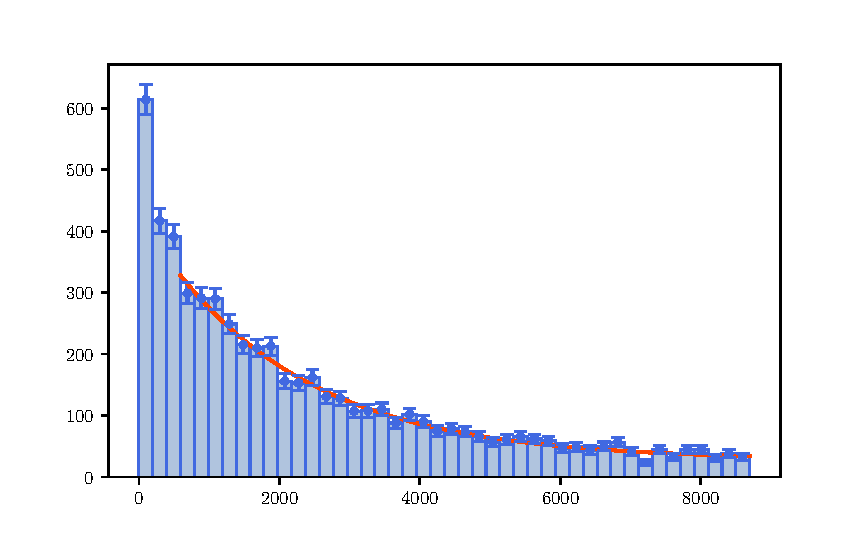
\includegraphics[width=0.6\textwidth]{plots/pALL.pdf}
    \caption{Measured events in all planes with plotted decay function.}
    \label{fig:pALL}
\end{figure}

The final result is 

\begin{align*}
    \tau = (2.1 \pm 0.1) \; \symup{\mu s}.
\end{align*} 

\section{Decay of captured muons}

\label{sec:muoncapture}

Since the muon has, apart from its mass, the same features as an electron, 
there is a probability for atoms capturing negative muons, which can influence
the outcome of this experiment, as discussed before. \\
Since the muon is in a bound state and thus under the influence of binding energy, 
the phase space for the decay gets reduced. A second effect is the relativistic time dilation due to the orbital movement of the muon. Both of these effects lead to a reduction in the decay rate of the bound state compared to the free state of the muon. A third effect is the Compton effect of the emitted electron, which can (virtually) interact with the atomic nucleus and therefore increases the decay rate of the bound muon compared to free muons. Considering these effects, the decay time for bound muons has to be modified\cite{bound}.\\

The time interval measured by this experiment also covers the area of times of the decay of captured muons in iron atoms which is $\tau_{\text{iron}} = 0.206 \; \symup{\mu s}$\cite{lvd}.
Only negative muons can get captured by the iron atoms. So, for simplicity, these analyses assume that all positive muons decay freely while most negative muons are captured by the material.
Because of this the fit function \ref{eqn:fit} can be adapted to 

\begin{equation*}
    N(t) = a \cdot \left( \frac{N_{+}}{N_{-}}\exp\left(- \frac{t}{\tau_{+}}\right) + \exp\left(- \frac{t}{\tau_{-}}\right) \right)  + b 
\end{equation*}

where $\tau_{+}$ is the decay time of the free decaying positive muons and $\tau_{-}$ is the decay time 
of the captured negative muons. The fraction $\frac{N_{+}}{N_{-}}$ describes the rate of 
positive muons over negative muons reaching the surface of the earth. In this analyisis this 
value will be assumed to be $\frac{N_{+}}{N_{-}} \approx 1.2$ \cite{lvd}. To have 
the most statistic the events of all planes in 59 bins will be used. The used event data and 
the plotted fit is shown in \autoref{fig:ptest}.

\begin{figure}
	 \centering
	 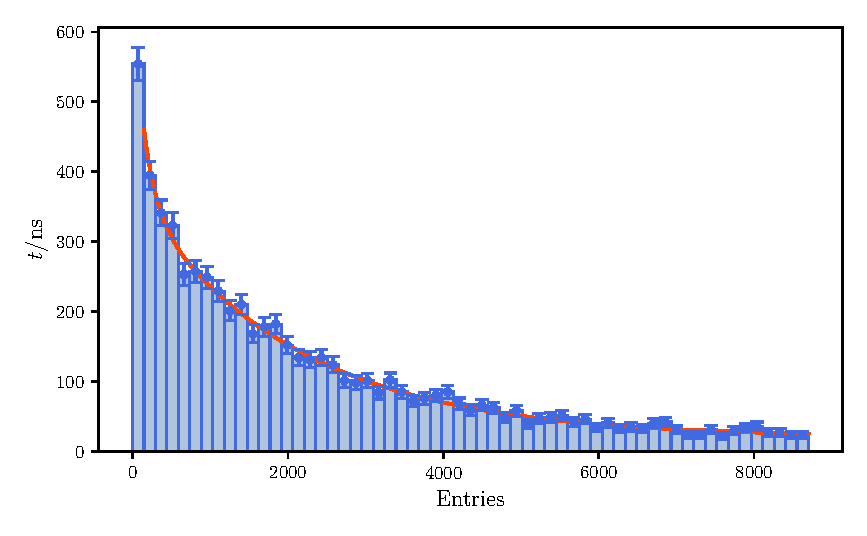
\includegraphics[width=0.6\textwidth]{plots/ptest.pdf}
	 \caption{Measured events in all planes with plotted modified decay function for captured muons.}
	 \label{fig:ptest}
\end{figure}
	
The calculated fit parameter are
	\begin{align*}
	 a &= 255 \pm 11\\
	 b &= 22 \pm 2 \\
	 \tau_{\text{+}} &= (1.9 \pm 0.1) \; \symup{\mu s}\\
	 \tau_{\text{-}} &= (0.15 \pm 0.04) \; \symup{\mu s}
	\end{align*}
with a test value of $\chi^2 = 0.89$ per degree of freedom.
